% Figure 1 (v16): v15 without the pack/citation subtitles, plus a light branch that shows external
% misconception evidence from the audit on the card (not passed to the evidence pack or the LLM).
% Figure 1 (v15): v14 with tidier routing: short response-log input to the behavioural summaries,
% held-out line turns inside Stage 2 (one clean crossing with the candidate-group line).
% Figure 1 (v14): Stage 1 as v12; Stage 2 redesigned around the audited candidate group.
% Audited candidate group -> representative distractors (content evidence) and behavioural summaries
% (learner-response context, also fed by the response logs) -> evidence pack -> LLM interpretation ->
% citation audit -> evidence-linked card (one per group) -> human evaluation (RQ2).
% Held-out assignment (RQ3) branches directly from semantic clustering.
% Compile: pdflatex fig1_pipeline_v14.tex
\documentclass[border=4pt]{standalone}
\usepackage{newtxtext}
\usepackage{tikz}
\usetikzlibrary{calc,arrows.meta,backgrounds}
\definecolor{semF}{RGB}{226,236,249}\definecolor{semD}{RGB}{88,120,170}
\definecolor{behF}{RGB}{251,234,220}\definecolor{behD}{RGB}{190,120,70}
\definecolor{bandA}{RGB}{246,248,251}\definecolor{bandB}{RGB}{250,248,245}
\newcommand{\sub}[1]{{\footnotesize\color{black!65}#1}}

\begin{document}
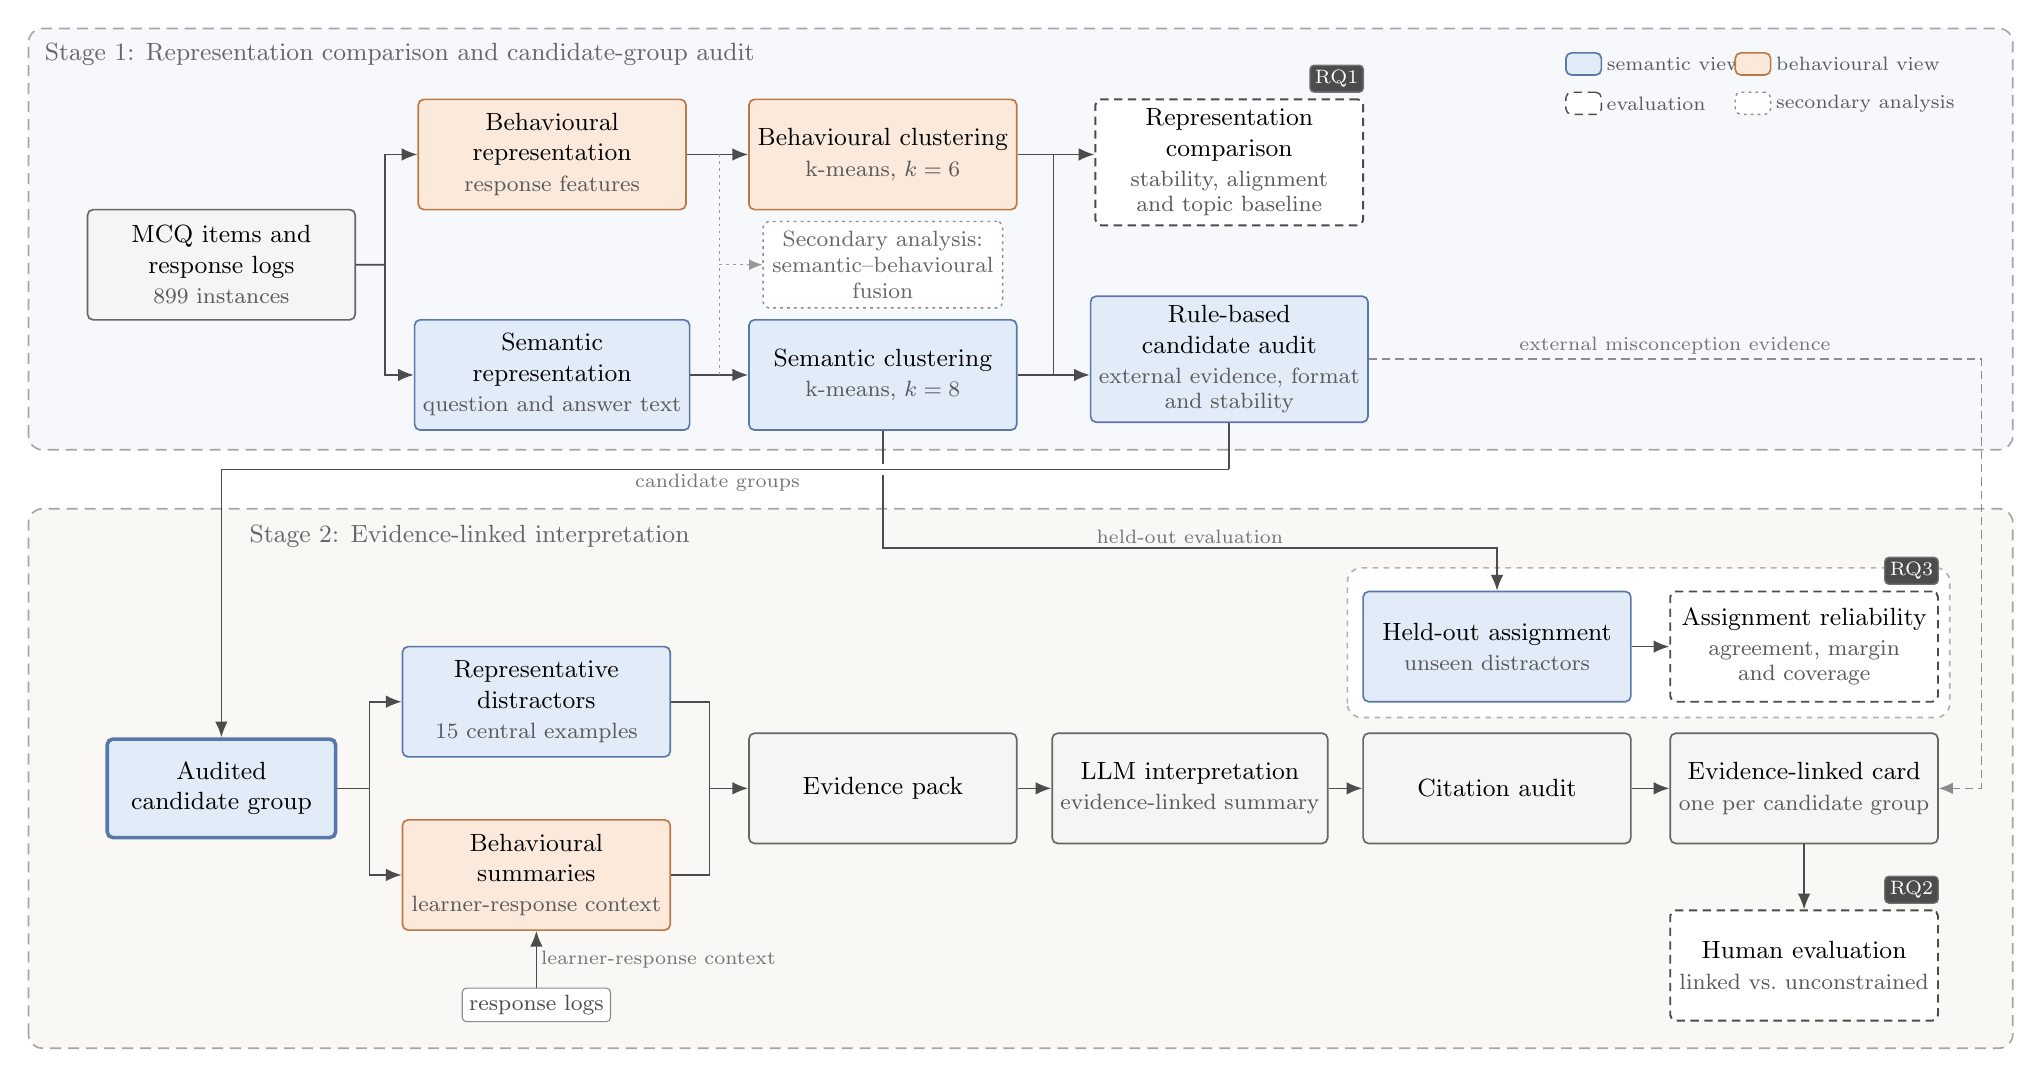
\begin{tikzpicture}[
  font=\small,
  box/.style={draw=black!60, line width=0.6pt, fill=white, rounded corners=2pt, align=center,
              minimum width=3.4cm, inner xsep=3pt, minimum height=1.4cm},
  sem/.style={box, fill=semF, draw=semD},
  beh/.style={box, fill=behF, draw=behD},
  proc/.style={box, fill=black!4},
  eval/.style={box, fill=white, draw=black!70, dash pattern=on 3pt off 2pt, line width=0.7pt},
  aux/.style={draw=black!45, line width=0.5pt, dash pattern=on 1pt off 1.5pt, fill=white, rounded corners=2pt, align=center,
              minimum width=3.0cm, minimum height=0.8cm, font=\footnotesize, text=black!60},
  rq/.style={draw=black!55, line width=0.5pt, rounded corners=1.5pt, fill=black!70, font=\scriptsize, text=white, inner sep=1.8pt},
  arr/.style={-{Latex[length=2.0mm, width=1.6mm]}, draw=black!70, line width=0.6pt},
  ln/.style={draw=black!70, line width=0.6pt},
  aarr/.style={-{Latex[length=1.7mm, width=1.4mm]}, draw=black!40, line width=0.5pt, dash pattern=on 1pt off 1.5pt},
  aln/.style={draw=black!40, line width=0.5pt, dash pattern=on 1pt off 1.5pt},
  band/.style={rounded corners=5pt, dash pattern=on 4pt off 2.5pt, line width=0.6pt},
  stage/.style={font=\small, text=black!60, inner sep=0pt},
  note/.style={font=\scriptsize, text=black!55, inner sep=1.5pt},
]
% ---------------- grid (cm)
\def\ca{0}\def\cb{4.2}\def\cc{8.4}\def\cd{12.8}
\def\ybeh{3.2}\def\ysem{0.4}\def\ymid{1.8}
\def\yt{-0.8}\def\yh{-1.8}
\def\yA{-3.75}\def\yM{-4.85}\def\yB{-5.95}\def\yL{-7.6}\def\yH{-3.05}\def\yE{-7.1}
\def\xg{0}\def\xe{4.0}\def\xp{8.4}\def\xl{12.3}\def\xa{16.2}\def\xk{20.1}
\def\R{22.75}

% ---------------- stage regions
\begin{scope}[on background layer]
  \filldraw[band, fill=bandA, draw=black!35] (-2.45,-0.55) rectangle (\R,4.8);
  \filldraw[band, fill=bandB, draw=black!35] (-2.45,-8.15) rectangle (\R,-1.3);
  \filldraw[band, fill=white, draw=black!30, dash pattern=on 2pt off 2pt] (14.3,-3.95) rectangle (21.95,-2.05);
\end{scope}
\node[stage, anchor=north west] at (-2.25,4.62) {Stage 1: Representation comparison and candidate-group audit};
\node[stage, anchor=north west] at (0.35,-1.5) {Stage 2: Evidence-linked interpretation};


% legend
\node[sem, minimum width=0.45cm, minimum height=0.28cm, inner sep=0pt] (lg1) at (17.3,4.35) {};
\node[note, anchor=west, text=black!65] at (lg1.east) {semantic view};
\node[beh, minimum width=0.45cm, minimum height=0.28cm, inner sep=0pt] (lg2) at (19.45,4.35) {};
\node[note, anchor=west, text=black!65] at (lg2.east) {behavioural view};
\node[eval, minimum width=0.45cm, minimum height=0.28cm, inner sep=0pt, line width=0.5pt] (lg3) at (17.3,3.85) {};
\node[note, anchor=west, text=black!65] at (lg3.east) {evaluation};
\node[aux, minimum width=0.45cm, minimum height=0.28cm, inner sep=0pt] (lg4) at (19.45,3.85) {};
\node[note, anchor=west, text=black!65] at (lg4.east) {secondary analysis};

% ---------------- Stage 1 (as v12)
\node[proc] (logs) at (\ca,\ymid) {MCQ items and\\ response logs\\ \sub{899 instances}};
\node[beh] (behf) at (\cb,\ybeh) {Behavioural\\ representation\\ \sub{response features}};
\node[sem] (semf) at (\cb,\ysem) {Semantic\\ representation\\ \sub{question and answer text}};
\node[beh] (behc) at (\cc,\ybeh) {Behavioural clustering\\ \sub{k-means, $k = 6$}};
\node[sem] (semc) at (\cc,\ysem) {Semantic clustering\\ \sub{k-means, $k = 8$}};
\node[eval, minimum height=1.6cm] (cmp) at (\cd,\ybeh-0.1) {Representation\\ comparison\\ \sub{stability, alignment}\\[-2pt] \sub{and topic baseline}};
\node[rq, anchor=south east] at ([yshift=2pt]cmp.north east) {RQ1};
\node[sem, minimum height=1.6cm] (aud) at (\cd,\ysem+0.2) {Rule-based\\ candidate audit\\ \sub{external evidence, format}\\[-2pt] \sub{and stability}};
\node[aux] (comb) at (\cc,\ymid) {Secondary analysis:\\ semantic--behavioural\\ fusion};

\coordinate (split) at ($(logs.east)!0.5!(semf.west |- logs.east)$);
\draw[ln]  (logs.east) -- (split);
\draw[arr] (split) |- (behf.west);
\draw[arr] (split) |- (semf.west);
\draw[arr] (behf.east) -- (behc.west);
\draw[arr] (semf.east) -- (semc.west);
\coordinate (cb) at ($(semf.east)!0.5!(semc.west)$);
\draw[aln]  (cb |- behf.east) -- (cb |- comb.west);
\draw[aln]  (cb) -- (cb |- comb.west);
\draw[aarr] (cb |- comb.west) -- (comb.west);
\coordinate (ch) at ($(semc.east)!0.5!(semc.east -| aud.west)$);
\draw[arr] (behc.east) -- (behc.east -| cmp.west);
\draw[arr] (semc.east) -- (semc.east -| aud.west);
\draw[ln]  (ch) -- (ch |- behc.east);

% ---------------- Stage 2: the audited candidate group is the unit
\node[sem, line width=1.3pt, minimum width=2.9cm, minimum height=1.25cm] (grp) at (\xg,\yM) {Audited\\ candidate group};
\node[sem] (rep)  at (\xe,\yA) {Representative\\ distractors\\ \sub{15 central examples}};
\node[beh] (bsum) at (\xe,\yB) {Behavioural\\ summaries\\ \sub{learner-response context}};
\node[proc] (pack)  at (\xp,\yM) {Evidence pack};
\node[proc] (llm)   at (\xl,\yM) {LLM interpretation\\ \sub{evidence-linked summary}};
\node[proc] (caud)  at (\xa,\yM) {Citation audit};
\node[proc] (card)  at (\xk,\yM) {Evidence-linked card\\ \sub{one per candidate group}};
\node[eval] (human) at (\xk,\yE) {Human evaluation\\ \sub{linked vs.\ unconstrained}};
\node[rq, anchor=south east] at ([yshift=2pt]human.north east) {RQ2};

% held-out branch (RQ3), directly from semantic clustering
\node[sem] (held) at (\xa,\yH) {Held-out assignment\\ \sub{unseen distractors}};
\node[eval] (rel)  at (\xk,\yH) {Assignment reliability\\ \sub{agreement, margin}\\[-2pt] \sub{and coverage}};
\node[rq, anchor=south east] at ([yshift=2pt]rel.north east) {RQ3};
\draw[arr] (semc.south) -- (\cc,\yh) -| (held.north);
\node[note, anchor=south] at ($(\cc,\yh)!0.5!(held.north |- 0,\yh)$) {held-out evaluation};
\draw[arr] (held.east) -- (rel.west);

% audit -> audited candidate group (passes over the held-out line with a gap)
\coordinate (tj) at (\cd,\yt);
\draw[white, line width=4pt] (\cc-0.12,\yt) -- (\cc+0.12,\yt);
\draw[ln]  (aud.south) -- (tj);
\draw[arr] (tj) -| (grp.north);
\node[note, anchor=north] at ($(\cc,\yt)!0.5!(\cb,\yt)$) {candidate groups};

% group -> content evidence and learner-response context
\coordinate (gf) at ($(grp.east)!0.5!(grp.east -| rep.west)$);
\draw[ln]  (grp.east) -- (gf);
\draw[arr] (gf) |- (rep.west);
\draw[arr] (gf) |- (bsum.west);

% response logs -> behavioural summaries (short input from below)
\node[note, draw=black!45, fill=white, rounded corners=1.5pt, inner sep=2.5pt, text=black!70, font=\footnotesize] (rl) at (\xe,\yL) {response logs};
\draw[arr] (rl.north) -- (bsum.south);
\node[note, anchor=west] at ($(rl.north)!0.5!(bsum.south)$) {learner-response context};

% evidence converges into the pack, then the interpretation chain
\coordinate (pf) at ($(rep.east)!0.5!(rep.east -| pack.west)$);
\draw[ln]  (rep.east) -- (pf) -- (pf |- pack.west);
\draw[ln]  (bsum.east) -- (bsum.east -| pf) -- (pf |- pack.west);
\draw[arr] (pf |- pack.west) -- (pack.west);
\draw[arr] (pack.east) -- (llm.west);
\draw[arr] (llm.east) -- (caud.west);
\draw[arr] (caud.east) -- (card.west);
\draw[arr] (card.south) -- (human.north);

% external misconception evidence: shown on the card, not passed to the evidence pack or the LLM
\coordinate (xr) at (22.35,0);
\draw[-{Latex[length=1.8mm, width=1.5mm]}, draw=black!45, line width=0.55pt, dash pattern=on 3pt off 1.8pt]
  (aud.east) -- (aud.east -| xr) -- (xr |- card.east) -- (card.east);
\node[note, anchor=south] at ($(aud.east)!0.5!(aud.east -| xr)$) {external misconception evidence};
\end{tikzpicture}
\end{document}
